\documentclass{standalone}

\usepackage{tikz}

\usetikzlibrary{shapes,
  shadings,
  calc,
  arrows,
  backgrounds,
  colorbrewer,
  shadows.blur}

% bold math smbols
\usepackage{bm}

% colors
\usepackage{xcolor}
\definecolor{TUanthrazit}{RGB}{50, 65, 75}


% from https://tex.stackexchange.com/a/216159
\newcommand{\cube}[1]{
  \begin{tikzpicture}
    % Settings
    \coordinate (CenterPoint) at (0,0);
    \def\width{0.7cm};
    \def\height{0.7cm};
    \def\textborder{0.1cm};
    \def\xslant{0.25cm};
    \def\yslant{0.15cm};
    \def\rounding{0.2pt};
    % Drawing
    \node[draw=white, draw,
    minimum height  = \height,
    minimum width   = \width,
    text width      = {\width-2*\textborder},
    align           = center,
    fill opacity    = 0.9,
    fill            = TUanthrazit!50,
    rounded corners = \rounding]
    (front)
    at (CenterPoint) {#1};
    % overlay front with Hessian silhouette
    \begin{pgfonlayer}{background}
      \node [inner sep=0pt] at (front) {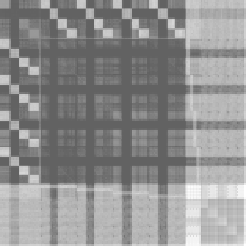
\includegraphics[width=\width]{hessian.pdf}};
    \end{pgfonlayer}
    % "3D" top
    \draw [rounded corners = \rounding, draw=white, fill=TUanthrazit!70] %
    ($(CenterPoint) + (-\width/2. - 2*\rounding, \height/2.)$) -- %
    ($(CenterPoint) + (-\width/2. + \xslant - 2*\rounding, \height/2. + \yslant)$) -- %
    ($(CenterPoint) + (\width/2. + \xslant + 2*\rounding, \height/2. + \yslant)$) -- %
    ($(CenterPoint) + (\width/2. + 2*\rounding, \height/2.)$) -- %
    cycle;
    % "3D" side
    \draw [rounded corners = \rounding, draw=white, fill=TUanthrazit!90] %
    ($(CenterPoint) + (\width/2. + \xslant + 2*\rounding, \height/2. + \yslant)$) -- %
    ($(CenterPoint) + (\width/2. + 2*\rounding, \height/2.)$) -- %
    ($(CenterPoint) + (\width/2. + 2*\rounding, -\height/2.)$) -- %
    ($(CenterPoint) + (\width/2. + \xslant + 2*\rounding, -\height/2. + \yslant)$) -- %
    cycle;
  \end{tikzpicture}
}

\begin{document}

\begin{tikzpicture}
  \node [inner sep=1pt] (A) {\cube{$\bm{A}$}};

  \node [anchor=south east, xshift=1.05cm, yshift=0.0cm] (v) at (A.north west)
  {\textbf{cur}$\bm{v}_{
\includegraphics[height=0.15cm]{torch.pdf}}$\textbf{linops}};

  \node (Av) [anchor=north west, xshift=-1ex, yshift=0.2cm] at (A.south east)
  {$\bm{Av}_{
\includegraphics[height=0.15cm]{torch.pdf}}$};

  \draw [->, >=stealth, thick] ($(v.south)+(-2ex,0)$) |- (A.west);

  \draw [->, >=stealth, thick] (A.east) -| (Av.north);
\end{tikzpicture}

\end{document}
